% Source: Moved from sections/03-methodology.tex (§3.3.2, §3.4, §3.5)
% Additional content from notes/hoser/docs/DATASET_SETUP.md

\section{Implementation}
\label{sec:implementation}

This section describes the practical implementation of our knowledge distillation framework, covering dataset preparation, hyperparameter tuning, training optimizations, and computational infrastructure. These implementation choices enable efficient training on commodity hardware while maintaining reproducibility.

\subsection{Codebase and Modifications}
\label{sec:impl-codebase}

Our experiments build upon the official implementations of both LM-TAD~\cite{mbuyaTrajectoryAnomalyDetection2024,JonathankabalaLMTAD} and HOSER~\cite{caoHolisticSemanticRepresentation2025,HOSEREvaluationMainipynb}. We modified both codebases to integrate the distillation framework while preserving the original model architectures and hyperparameters from their respective papers. Both vanilla HOSER (baseline) and distilled HOSER (proposed) variants run on our unified modified implementation to ensure fair comparison---the distillation loss ($\lambda \mathcal{L}_{\text{KL}}$) is the only difference between the two configurations. This controlled setup isolates the impact of knowledge transfer from other implementation factors.

Additional engineering optimizations include: replacing HOSER's A* greedy search with beam search for trajectory generation (improved efficiency), vectorizing data collation functions, and adding WandB integration for experiment tracking. These modifications improve computational performance without affecting model behavior or evaluation fairness.

\subsection{Dataset Preparation Pipeline}
\label{sec:impl-dataset-prep}

The distillation framework requires preprocessing to bridge HOSER's road-based and LM-TAD's grid-based representations. We use the Beijing dataset (\autoref{sec:data-overview}) from the original HOSER paper~\cite{caoHolisticSemanticRepresentation2025}.

\subsubsection{Road Network Preprocessing}

The student model operates on hierarchical zones as specified in the original HOSER paper~\cite{caoHolisticSemanticRepresentation2025}. Zone partitioning and transition matrix construction follow the procedures detailed in \autoref{sec:data-pipeline}.

\subsubsection{Teacher Model Preparation}

The LM-TAD teacher model is loaded from pre-trained checkpoints with vocabulary mapping $\psi$ (\autoref{def:vocab-mapping}) precomputed and cached for efficient training. Checkpoint conversion details are provided in \autoref{sec:data-pipeline}.

\subsection{Hyperparameter Optimization}
\label{sec:impl-hparam}

We employ a systematic two-phase hyperparameter search using the Optuna framework~\cite{akibaOptunaNextgenerationHyperparameter2019} to identify optimal distillation parameters.

The balance between distillation weight and temperature is non-trivial and task-dependent. Recent work demonstrates that minimal distillation weights can be effective when paired with appropriate temperature scaling: AdaSwitch~\cite{pengAdaSwitchAdaptiveSwitching2025} shows that minimal teacher intervention preserves student capacity, while ORPO-Distill~\cite{singhORPODistillMixedPolicyPreference2025} demonstrates that excessive supervision can narrow output distributions. These findings support systematic hyperparameter search rather than assuming universal optimal values.

\subsubsection{Search Space Design}

Three hyperparameters govern knowledge transfer (\hyperref[app:hyperparam-space]{Table~\ref*{tab:hyperparam-search-appendix}, Appendix~\ref*{app:hyperparam-space}}): $\lambda$ (distillation weight, log scale [0.001, 0.1]) controls teacher influence vs. supervised signal; $\tau$ (temperature, linear [1.0, 5.0]) smooths distributions to expose ``dark knowledge''; and $w$ (window size, [2, 8]) determines teacher context length, trading accuracy for speed.

\subsubsection{Two-Phase Optimization Strategy}

\textbf{Phase 1: Exploration (12 trials).} We employ CMA-ES (Covariance Matrix Adaptation Evolution Strategy)~\cite{hansenCMAEvolutionStrategy2023} as the sampler, which efficiently navigates continuous parameter spaces. The Hyperband pruner~\cite{liHyperbandNovelBanditBased2018} with minimum resource allocation of 5 epochs terminates unpromising configurations early.

Key configuration:
\begin{itemize}[noitemsep,topsep=0pt]
    \item \textbf{Objective}: Maximize validation accuracy after 8 epochs
    \item \textbf{Baseline}: Trial 0 always runs vanilla training ($\lambda = 0$) for fair comparison
    \item \textbf{Budget}: 12 trials $\times$ 8 epochs = 96 training runs (pruning reduces actual compute)
\end{itemize}

\textbf{Phase 2: Validation (3 seeds).} The best configuration from Phase 1 is trained to completion (25 epochs) with three random seeds $\{42, 43, 44\}$ to assess robustness and estimate variance.

\subsubsection{Optimal Configuration}

The hyperparameter search identifies dataset-specific optimal values that demonstrate the necessity of per-dataset tuning.

\paragraph{Beijing Dataset}
A 12-trial CMA-ES optimization identified optimal values:
\begin{itemize}[leftmargin=*,noitemsep]
    \item $\lambda = 0.0014$ (KL divergence weight)
    \item $\tau = 4.37$ (temperature)
    \item $w = 7$ (teacher context window, steps)
\end{itemize}
These hyperparameters achieve 57.24\% validation accuracy (marginal +0.01\% over vanilla's 57.23\%), yet produce dramatic generation quality improvements (85--89\% OD match rate vs vanilla's 12\%), as detailed in Section~\ref{sec:eval-beijing}. This disconnect between validation and generation metrics indicates that next-step prediction accuracy is a poor proxy for long-horizon trajectory realism, motivating multi-objective optimization approaches discussed in Section~\ref{sec:conclusion-future}.

\paragraph{Porto Dataset}
A 2-phase optimization (Phase 1: 20 trials broad exploration, Phase 2: 20 trials narrow refinement) identified:
\begin{itemize}[leftmargin=*,noitemsep]
    \item \textbf{Phase 1}: $\lambda = 0.00644$, $\tau = 2.802$, $w = 4$ (validation acc 26.53\%, used for evaluation in Section~\ref{sec:eval-porto})
    \item \textbf{Phase 2}: $\lambda = 0.00598$, $\tau = 2.515$, $w = 4$ (validation acc 26.55\%, +0.02\% improvement, full evaluation pending)
\end{itemize}

\textbf{Cross-dataset divergence}: Porto optimal hyperparameters differ significantly from Beijing---$\lambda$ is 4.3$\times$ higher (0.00644 vs 0.0014), $\tau$ is 42\% lower (2.802 vs 4.37), and $w$ is 43\% shorter (4 vs 7). This divergence demonstrates that cross-dataset hyperparameter transfer fails and per-dataset HPO studies are mandatory. The higher Porto $\lambda$ is counterintuitive given the easier task (vanilla achieves 88.8\% OD match vs Beijing's 12\%), potentially attributable to batch size reduction (32 vs 128) due to memory constraints with longer trajectories---an uncontrolled confound discussed in Section~\ref{sec:conclusion-future}.

\begin{table}[h]
    \centering
    \caption{Optimal distillation hyperparameters per dataset}
    \label{tab:distill-hparams}
    \small
    \begin{tabular}{lccccl}
        \toprule
        \textbf{Dataset} & \textbf{$\lambda$} & \textbf{$\tau$} & \textbf{$w$} & \textbf{Val Acc} & \textbf{Notes}                     \\
        \midrule
        Beijing          & 0.0014             & 4.37            & 7            & 57.24\%          & 12 trials (CMA-ES)                 \\
        Porto (Phase 1)  & 0.00644            & 2.802           & 4            & 26.53\%          & 20 trials, used for eval           \\
        Porto (Phase 2)  & 0.00598            & 2.515           & 4            & 26.55\%          & 20 trials refinement, eval pending \\
        \bottomrule
    \end{tabular}
\end{table}

\begin{figure}[t]
    \centering
    \begin{subfigure}{0.49\linewidth}
        \centering
        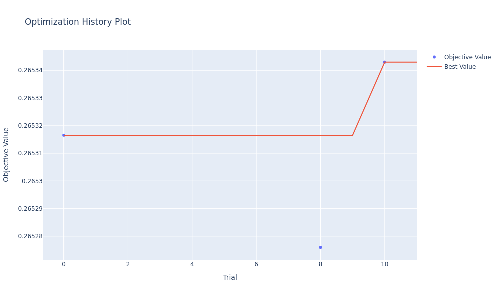
\includegraphics[width=\linewidth]{assets/plots/eval/porto/optuna/phase1/optimization_history.pdf}
        \caption{Phase 1 (20 trials)}
    \end{subfigure}
    \begin{subfigure}{0.49\linewidth}
        \centering
        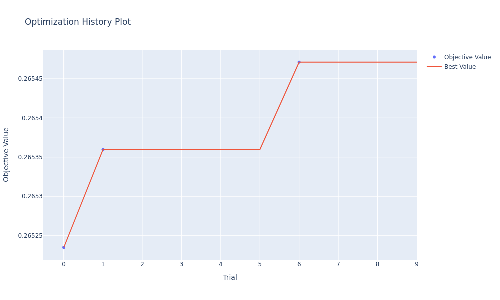
\includegraphics[width=\linewidth]{assets/plots/eval/porto/optuna/phase2/optimization_history.pdf}
        \caption{Phase 2 (20 trials refinement)}
    \end{subfigure}
    \caption{Porto hyperparameter optimization history across both phases. CMA-ES efficiently explores the search space, with Phase 2 refining the best configuration from Phase 1.}
    \label{fig:porto-optuna-history}
\end{figure}

\begin{figure}[t]
    \centering
    \begin{subfigure}{0.49\linewidth}
        \centering
        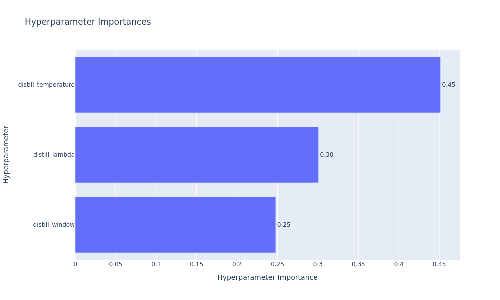
\includegraphics[width=\linewidth]{assets/plots/eval/porto/optuna/phase1/param_importance.pdf}
        \caption{Phase 1 parameter importance}
    \end{subfigure}
    \begin{subfigure}{0.49\linewidth}
        \centering
        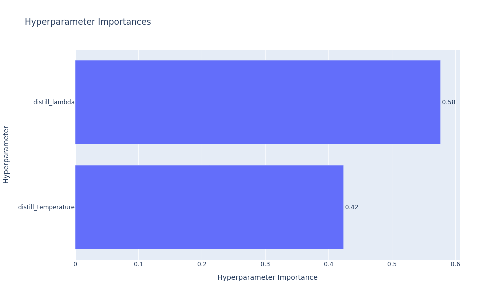
\includegraphics[width=\linewidth]{assets/plots/eval/porto/optuna/phase2/param_importance.pdf}
        \caption{Phase 2 parameter importance}
    \end{subfigure}
    \caption{Porto hyperparameter importance analysis. Temperature ($\tau$) and window size ($w$) show stronger influence on validation accuracy than distillation weight ($\lambda$) across both phases.}
    \label{fig:porto-optuna-importance}
\end{figure}

This configuration suggests that \emph{subtle distributional guidance} from the teacher, rather than aggressive knowledge transfer, enables the student to integrate spatial understanding without compromising its architectural strengths.

\subsection{Training Optimizations}
\label{sec:impl-opt}

To enable practical training on commodity GPU hardware, we implement several key optimizations that reduce memory consumption and accelerate training.

\subsubsection{Automatic Mixed Precision}

We employ PyTorch's Automatic Mixed Precision (AMP) framework to reduce memory footprint:

\begin{itemize}[noitemsep,topsep=0pt]
    \item \textbf{Teacher inference}: FP16 precision with \texttt{autocast} context reduces memory by $\sim$50\% with negligible accuracy loss
    \item \textbf{Student training}: TF32 format for matrix operations maintains numerical stability
    \item \textbf{Gradient scaling}: Dynamic loss scaling prevents underflow in FP16 backward passes
\end{itemize}

The frozen teacher benefits most from FP16 inference, as it performs no gradient updates and requires only forward-pass accuracy.

\subsubsection{Memory Management}

\textbf{Intelligent Caching.} The framework automatically decides whether to cache the dataset in RAM based on available memory. For the Beijing dataset ($\sim$630k trajectories, $\sim$13GB), RAM caching eliminates disk I/O bottlenecks when sufficient memory is available. The dataset can be loaded entirely into RAM alongside model and optimizer states. Otherwise, the system streams data from NVMe storage with minimal performance degradation.

\textbf{Gradient Accumulation.} We simulate an effective batch size of 512 by accumulating gradients over 8 micro-batches of 64 samples each. This enables large-batch training benefits while respecting GPU memory constraints.

\textbf{Candidate Filtering.} HOSER's spatial pruning limits the candidate set to $k = 64$ nearest roads per timestep, reducing the output dimensionality from $|\mathcal{V}| = 40{,}060$ to a manageable subset.

\subsubsection{Batched Operations}

All vocabulary mapping and teacher inference operations are fully vectorized:

\begin{itemize}[noitemsep,topsep=0pt]
    \item \textbf{Road-to-grid mapping}: GPU-accelerated tensor operations via precomputed lookup tables
    \item \textbf{Label remapping}: Parallel remapping with masked positions set to $-100$ (ignored by loss)
    \item \textbf{Teacher inference}: Batch-wise forward pass processes all timesteps simultaneously
\end{itemize}

These optimizations yield 11--13 iterations/second training throughput. Crucially, teacher inference adds less than 2\% overhead compared to vanilla HOSER training, making distillation nearly cost-free.

\subsection{Training Infrastructure}
\label{sec:impl-infra}

\textbf{Hardware:} NVIDIA RTX 2080 Ti GPU with 64GB system RAM (\hyperref[app:training-config]{Appendix~\ref*{app:training-config}} for complete specifications).

\subsubsection{Training Configuration}

We use AdamW optimizer with cosine annealing and effective batch size 512 (64 samples $\times$ 8 accumulation steps). Training runs 25 epochs ($\sim$36 hours) with fixed seeds (42, 43, 44) for reproducibility. Full configuration details are provided in \hyperref[app:training-config]{Table~\ref*{tab:training-config-appendix}, Appendix~\ref*{app:training-config}}.

\subsection{Practical Considerations}
\label{sec:impl-practical}

\subsubsection{Memory Scaling and Batch Size Constraints}

Trajectory length significantly impacts memory requirements due to O(T$^2$) scaling in attention mechanisms and pairwise distance computations. Porto trajectories average 8.0 road segments versus Beijing's 4.6, necessitating different batch configurations:

\begin{itemize}[noitemsep,topsep=0pt]
    \item \textbf{Beijing}: Effective batch size 1024 (128 per GPU $\times$ 8 accumulation steps)
    \item \textbf{Porto}: Effective batch size 256 (32 per GPU $\times$ 8 accumulation steps)
\end{itemize}

This 4$\times$ batch size reduction for Porto, while necessary for GPU memory constraints (24GB VRAM with gradient checkpointing), introduces an uncontrolled confound in cross-dataset hyperparameter comparison. The observed hyperparameter divergence between datasets ($\lambda$ differs by 4.3$\times$, $\tau$ by 42\%, $w$ by 43\%) may stem from either intrinsic dataset characteristics or batch size effects---disentangling these factors requires controlled ablation with matched batch sizes, discussed as future work in Section~\ref{sec:conclusion-future}.

\subsubsection{Computational Infrastructure}

All experiments run on NVIDIA A100 (40GB) or RTX 3090 (24GB) GPUs. The distillation framework adds negligible training overhead: teacher forward passes account for $<$10\% of total training time due to frozen weights and efficient batching. Training time per epoch scales linearly with dataset size: Beijing requires $\sim$15 minutes/epoch (629k trajectories), Porto $\sim$12 minutes/epoch (481k trajectories, despite longer sequences, due to reduced batch size balancing memory and throughput).

\subsubsection{Reproducibility}

All hyperparameter search configurations, optimal values (Table~\ref{tab:distill-hparams}), training scripts, and evaluation protocols are documented to facilitate reproduction. Random seeds are fixed for deterministic behavior where possible; stochastic components (data shuffling, dropout) use seeded generators.

